\chapterimage{oilseed-mill} % Chapter heading image

\chapter{Ponteiros e Alocação Dinâmica de Memória}
Há momentos em que é conveniente alocar memória em tempo de execução usando \textbf{malloc()}, \textbf{calloc()} ou outras funções de alocação. O uso dessa abordagem permite adiar a decisão sobre o tamanho do bloco de memória necessário para armazenar um \textit{array}, por exemplo, até o tempo de execução. Ou permite usar uma seção de memória para o armazenamento de um \textit{array} de inteiros em um ponto no tempo, e então quando essa memória não for mais necessária, ela pode ser liberada para outros usos, como o armazenamento de um \textit{array} de estruturas.

Quando a memória é alocada, a função de alocação (como \textbf{malloc()}, \textbf{calloc()}, etc.) retorna um ponteiro. O tipo deste ponteiro depende se você está usando um compilador \textbf{K\&R} mais antigo ou o compilador mais recente. Com o compilador mais antigo, o tipo do ponteiro retornado é \textbf{char}, com compiladores atuais é \textbf{void}.

Se você estiver usando um compilador mais antigo e quiser alocar memória para um \textit{array} de inteiros, terá que converter o ponteiro \textbf{char} retornado para um ponteiro inteiro. Por exemplo, para alocar espaço para 10 inteiros, podemos escrever:
\begin{lstlisting}
	int *iptr;
	iptr = (int *)malloc(10 * sizeof(int));
	if (iptr == NULL)
	{ .. A ROTINA DE ERROS VAI AQUI .. }
\end{lstlisting}

Se você estiver usando um compilador atual, \textbf{malloc()} retorna um ponteiro \textbf{void} e como um ponteiro \textbf{void} pode ser atribuído a uma variável de ponteiro de qualquer tipo de objeto, o \textit{cast} \textbf{(int *)} mostrado acima não é necessário: 
\begin{lstlisting}
	int *iptr;
	iptr = malloc(10 * sizeof(int));
\end{lstlisting}
A dimensão do \textit{array} pode ser determinada em tempo de execução e não é necessária em tempo de compilação. Ou seja, o 10 acima pode ser uma variável lida de um arquivo de dados ou teclado, ou calculada com base em alguma necessidade, em tempo de execução.

Por causa da equivalência entre a notação de \textit{array} e ponteiro, uma vez que \textbf{iptr} tenha sido atribuído como acima, pode-se usar a notação de \textit{array}. Por exemplo, pode-se escrever:
\begin{lstlisting}
	int k;
	for (k = 0; k < 10; k++)
		iptr[k] = 2;
\end{lstlisting}
para definir os valores de todos os elementos para 2.

Mesmo com um entendimento razoavelmente bom de ponteiros e \textit{arrays}, um lugar que o novato em C provavelmente tropeçará no início é na alocação dinâmica de \textit{arrays} multidimensionais. Em geral, gostaríamos de poder acessar elementos de tais \textit{arrays} usando notação de \textit{array}, não notação de ponteiro, sempre que possível. Dependendo da aplicação, podemos ou não saber as duas dimensões no momento da compilação. Isso nos leva a diversas maneiras de realizar nossa tarefa.

Como vimos, ao alocar dinamicamente um \textit{array} unidimensional, sua dimensão pode ser determinada em tempo de execução. Agora, ao usar a alocação dinâmica de \textit{arrays} de ordem superior, nunca precisamos saber a primeira dimensão em tempo de compilação. Se precisamos saber as dimensões superiores depende de como vamos escrever o código. Aqui, discutirei vários métodos de alocação dinâmica de espaço para \textit{arrays} bidimensionais de inteiros.

\section*{MÉTODO 1:}
Uma maneira de lidar com o problema é usando a palavra-chave \textbf{typedef}. Para alocar um \textit{array} bidimensional de inteiros, lembre-se de que as duas notações a seguir resultam na geração do mesmo código de objeto:
\begin{lstlisting}
	multi[lin][col] = 1;         // Usando array
	*(*(multi + lin) + col) = 1; // Usando ponteiro
\end{lstlisting}

Também é verdade que as duas notações a seguir geram o mesmo código:
\begin{lstlisting}
	multi[lin];     // Usando array
	*(multi + lin); // Usando ponteiro
\end{lstlisting}

Visto que a segunda linha deve ser avaliada como um ponteiro, a notação de \textit{array} da primeira linha também deve ser avaliada como um ponteiro. Na realidade, \textbf{multi[0]} retornará um ponteiro para o primeiro inteiro na primeira linha, \textbf{multi[1]} um ponteiro para o primeiro inteiro da segunda linha, etc. Na verdade, \textbf{multi[n]} avalia como um ponteiro para aquele \textit{array} de inteiros que constituem a enésima linha de nosso array bidimensional. Ou seja, \textbf{multi} pode ser pensado como um \textit{array} de \textit{arrays} e \textbf{multi[n]} como um ponteiro para o enésimo \textit{array} deste \textit{array} de \textit{arrays}. Aqui, a palavra ponteiro está sendo usada para representar um valor de endereço. Embora tal uso seja comum na literatura, ao ler tais declarações deve-se ter o cuidado de distinguir entre o endereço constante de um \textit{array} e um ponteiro de variável, que é um objeto de dados em si.

Considere agora:
\lstinputlisting[label=prog:ponteiros, caption=Ponteiros e malloc, numbers=left]{code/prog9-1.c}

Aqui, assumi um compilador atual, portanto, uma conversão no ponteiro \textbf{void} retornado por \textbf{malloc()} não é necessária. Se você estivesse usando um compilador \textbf{K\&R }mais antigo, teria que converter usando:
\begin{lstlisting}
	lptr = (ArrayLinha *)malloc(nlinhas * COLS * sizeof(int));
\end{lstlisting}

Usando esta abordagem, \textbf{lptr} tem todas as características de um nome de \textit{array}, (exceto que \textbf{lptr} é modificável), e a notação de \textit{array} pode ser usada em todo o resto do programa. Isso também significa que, se você pretende escrever uma função para modificar o conteúdo do \textit{array}, deve usar \textbf{COLS} como parte do parâmetro formal dessa função, assim como fizemos ao discutir a passagem de \textit{arrays} bidimensionais para uma função.

\section*{MÉTODO 2:}
No MÉTODO 1, \textbf{lptr} acabou sendo um ponteiro para tipo ``um array unidimensional de COLS inteiros''. Acontece que existe uma sintaxe que pode ser usada para esse tipo sem a necessidade de \textbf{typedef}. Se escrevermos:
\begin{lstlisting}
	int (*xptr)[COLS];
\end{lstlisting}
a variável \textbf{xptr} terá todas as características da variável \textbf{lptr} no \textbf{MÉTODO 1}, e não precisamos usar a palavra-chave \textit{typedef}. Aqui \textbf{xptr} é um ponteiro para um \textit{array} de inteiros e o tamanho desse \textit{array} é dado por \textbf{\#define COLS}. O posicionamento dos parênteses faz com que a notação de ponteiro predomine, embora a notação de \textit{array} tenha precedência mais alta. ou seja, se houvéssemos escrito
\begin{lstlisting}
	int *xptr[COLS];
\end{lstlisting}
teríamos definido \textbf{xptr} como um \textit{array} de ponteiros contendo o número de ponteiros igual ao \textbf{\#definido} por \textbf{COLS}. Isso não é a mesma coisa de forma alguma. No entanto, \textit{arrays} de ponteiros têm seu uso na alocação dinâmica de \textit{arrays} bidimensionais, como será visto nos próximos 2 métodos.

\section*{MÉTODO 3:}
Considere o caso em que não sabemos o número de elementos em cada linha em tempo de compilação, ou seja, o número de linhas e o número de colunas devem ser determinados em tempo de execução. Uma maneira de fazer isso seria criar um \textit{array} de ponteiros para o tipo \textbf{int} e então alocar espaço para cada linha e apontar esses ponteiros para cada linha. Considere:
\lstinputlisting[label=prog:metodo3, caption=Método 3, numbers=left]{code/prog9-2.c}

No código anterior, \textbf{ptrlinha} é um ponteiro de um ponteiro para o tipo \textbf{int}. Nesse caso, ele aponta para o primeiro elemento de um \textit{array} de ponteiros para o tipo \textbf{int}. Considere o número de chamadas para \textbf{malloc()}:

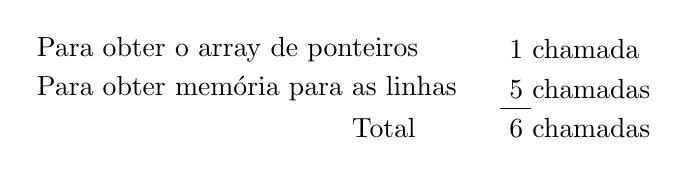
\begin{tikzpicture}
\node[anchor=west] at (0,0)    {Para obter o array de ponteiros};
\node[anchor=west] at (0,-0.5) {Para obter memória para as linhas};
\node[anchor=west] at (4,-1) {Total};
\node[anchor=west] at (6,0)    {1 chamada};
\node[anchor=west] at (6,-0.5) {5 chamadas};
\node[anchor=west] at (6,-1) {6 chamadas};
\draw (6,-0.75) -- (6.4,-0.75);
\end{tikzpicture}

Se você optar por usar esta abordagem, observe que, embora você possa usar a notação de \textit{array} para acessar elementos individuais do \textit{array}, por exemplo, \textbf{ptrlinha[lin][col] = 42;}, isso não significa que os dados no ``\textit{array} bidimensional'' são contíguos na memória.

Você pode, entretanto, usar a notação de \textit{array} como se fosse um bloco contínuo de memória. Por exemplo, você pode escrever:
\begin{lstlisting}
	ptrlinha[lin][col] = 176;
\end{lstlisting}
exatamente como se \textbf{ptrlinha} fosse o nome de um \textit{array} bidimensional criado em tempo de compilação. É claro que \textbf{lin} e \textbf{col} devem estar dentro dos limites do \textit{array} que você criou, assim como com um \textit{array} criado em tempo de compilação.

Se você deseja ter um bloco contíguo de memória dedicado ao armazenamento dos elementos do \textit{array}, pode fazê-lo da seguinte maneira:

\section*{MÉTODO 4:}
Neste método, alocamos um bloco de memória para armazenar primeiro o \textit{array} inteiro. Em seguida, criamos um \textit{array} de ponteiros para apontar para cada linha. Portanto, mesmo que o \textit{array} de ponteiros esteja sendo usado, o \textit{array} real na memória é contíguo. O código é parecido com este:
\lstinputlisting[label=prog:metodo4, caption=Método 4., numbers=left]{code/prog9-3.c}

Considere novamente, o número de chamadas para \textbf{malloc()}

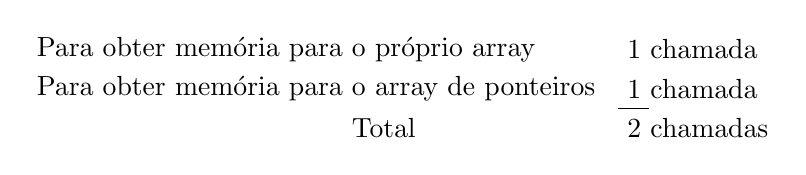
\begin{tikzpicture}
\node[anchor=west] at (0,0)    {Para obter memória para o próprio array};
\node[anchor=west] at (0,-0.5) {Para obter memória para o array de ponteiros};
\node[anchor=west] at (4,-1) {Total};
\node[anchor=west] at (7.5,0)    {1 chamada};
\node[anchor=west] at (7.5,-0.5) {1 chamada};
\node[anchor=west] at (7.5,-1) {2 chamadas};
\draw (7.5,-0.75) -- (7.9,-0.75);
\end{tikzpicture}

Agora, cada chamada para \textbf{malloc()} cria uma sobrecarga de espaço adicional, já que \textbf{malloc()} é geralmente implementado pelo sistema operacional formando uma lista encadeada que contém dados relativos ao tamanho do bloco. Mas, mais importante, com grandes arrays (várias centenas de linhas), controlar o que precisa ser liberado quando chega a hora pode ser mais complicado. Isso, combinado com a contiguidade do bloco de dados que permite a inicialização para todos os zeros usando \textbf{memset()}, parece tornar a segunda alternativa a preferida.

Como um exemplo final em \textit{arrays} multidimensionais, ilustraremos a alocação dinâmica de um \textit{array} tridimensional. Este exemplo ilustrará mais uma coisa a se observar ao fazer esse tipo de alocação. Pelas razões citadas anteriormente, usaremos a abordagem descrita na alternativa dois. Considere o seguinte código:
\lstinputlisting[label=prog:tridimensional, caption=Alocação de Array Tridimensional.., numbers=left]{code/prog9-4.c}

Se você seguiu este tutorial até este ponto, não deverá ter problemas para decifrar o programa \ref{prog:tridimensional} com base apenas nos comentários. No entanto, há alguns pontos que devem ser destacados. Vamos começar com a linha que diz:
\begin{lstlisting}
	Arr3D[z][y] = espaco + (z * (X_DIM * Y_DIM) + y * X_DIM);
\end{lstlisting}

Observe que aqui \textbf{espaço} é um ponteiro de caractere, que é do mesmo tipo que \textbf{Arr3D[z][y]}. É importante que ao adicionar um inteiro, como o obtido pela avaliação da expressão \textbf{(z * (X\_DIM * Y\_DIM) + y * X\_DIM)}, a um ponteiro, o resultado seja um novo valor do ponteiro. E ao atribuir valores de ponteiro a variáveis de ponteiro, os tipos de dados do valor e da variável devem corresponder.
